\ifx\handout\undefined
  \documentclass[compress,t,aspectratio=169]{beamer}
\else
  \documentclass[compress,handout,t,aspectratio=169]{beamer}
  \usepackage{pgfpages}
  %\pgfpagesuselayout{8 on 1}[letterpaper,border shrink=1mm]
  \pgfpagesuselayout{8 on 1}[letterpaper,border shrink=0mm]
\fi

\input{preamble}
\usepackage{multicol}
\usepackage{ulem} % used in definition of \redout

\usepackage{tikz}
\usetikzlibrary{arrows,snakes,backgrounds,shapes}
\tikzstyle{commit}=[circle,draw=blue!50,fill=blue!20]
\tikzstyle{redCommit}=[circle,draw=MyRed!50,fill=MyRed!20]
\tikzstyle{redConflict}=[circle,draw=MyRed!50,dashed,fill=MyRed!20]
\tikzstyle{orphanCommit}=[black!50,circle,draw=blue!20,fill=blue!10]
\tikzstyle{droppedCommit}=[black!60,circle,draw=MyRed!50,fill=MyRed!20,double]
\tikzstyle{ref}=[rectangle,draw=black!50,fill=black!20]
\tikzstyle{specialRef}=[black!50,rectangle,draw=black!50,fill=black!10]
\tikzstyle{msg}=[tape,tape bend top=none,draw=MyRed!50,fill=MyRed!20]
\tikzstyle{prnt}=[thick,-stealth']
\tikzstyle{oprnt}=[black!50,dotted,-stealth',draw=black!50]
\tikzstyle{bptrnext}=[black!80,dashed,-stealth',draw=black!80]
\tikzstyle{bptr}=[thick,-latex']
\tikzstyle{nextmsg}=[thick,-open triangle 45]
\newcommand{\parent}[1]{\char94{#1}}
\newcommand{\ancestor}[1]{\char126{#1}}
\colorlet{myred}{red!90!black} % slightly darker than normal red
\colorlet{myblue}{cyan}        % plain cyan works; might consdier darkening
\colorlet{mygreen}{green!70!black} % slightly darker than normal green
\colorlet{mypurple}{red!45!blue}
\definecolor{mybrown}{rgb}{0.45,0.28,0.13}
\newcommand\redout{\bgroup\markoverwith
    {\textcolor{myred}{\rule[.5ex]{2pt}{0.8pt}}}\ULon
}

\title{git-filter-repo for rewriting Git history}

\author{Elijah Newren}
\institute{GitHub}

%\date{September 19, 2024}
%\date{$O_2 \Rightarrow CO_2$ Conversion Specialist}
\date{}

\begin{document}

\begin{frame}
  \titlepage
\end{frame}

%%%%%%%%%%%%%%%%%%%%%%%%%%%%%%%%%%%%%%%%%%%%%%%%%%%%%%%%%%%%%%%%%%%%%%%%%%
\section[Introduction]{git-filter-repo overview}
\subsection{Purpose}
%%%%%%%%%%%%%%%%%%%%%%%%%%%%%%%%%%%%%%%%%%%%%%%%%%%%%%%%%%%%%%%%%%%%%%%%%%

\begin{frame}
  \frametitle{What is git-filter-repo}

  git-filter-repo is a versatile tool for rewriting Git History.
  \vspace*{\baselineskip}

  \pause
  Examples things it can be used for:
  \begin{itemize}[<+->]
    \item restructure file layout in history
    \begin{itemize}
      \item keep only a subset
      \item expunge a subset
      \item rename
    \end{itemize}
    \item modifying file contents throughout history
    \item rewrite commit messages
  \end{itemize}

\end{frame}

%%%%%%%%%%%%%%%%%%%%%%%%%%%%%%%%%%%%%%%%%%%%%%%%%%%%%%%%%%%%%%%%%%%%%%%%%%
\subsection{Usability touches}
%%%%%%%%%%%%%%%%%%%%%%%%%%%%%%%%%%%%%%%%%%%%%%%%%%%%%%%%%%%%%%%%%%%%%%%%%%

%%%%%%%%%%%%%%%%%%%%%%%%%%%%%%%%%%%%%%%%%%%%%%%%%%%%%%%%%%%%%%%%%%%%%%%%%%
\begin{frame}
  \frametitle{Taking care of the small details}

  git-filter-repo handles several important details automatically

  \begin{itemize}[<+->]
    \item updating references to commit hashes in commit messages
    \item pruning commits which become empty due to the filtering operation
    \item make replace refs (\texttt{refs/replace/...}) and grafts permanent
    \item rewriting stashes$^*$
    \item cleaning out the old history \& repacking
  \end{itemize}

\end{frame}

%%%%%%%%%%%%%%%%%%%%%%%%%%%%%%%%%%%%%%%%%%%%%%%%%%%%%%%%%%%%%%%%%%%%%%%%%%
\subsection{Public service announcements}
%%%%%%%%%%%%%%%%%%%%%%%%%%%%%%%%%%%%%%%%%%%%%%%%%%%%%%%%%%%%%%%%%%%%%%%%%%

%%%%%%%%%%%%%%%%%%%%%%%%%%%%%%%%%%%%%%%%%%%%%%%%%%%%%%%%%%%%%%%%%%%%%%%%%%
\begin{frame}
  \frametitle{Public service announcements}

  Important points to keep in mind:

  \begin{itemize}[<+->]
    \item \textit{Destructive by design}, but aborts by default if not in a
          fresh clone
    \item Extended commit headers, such as commit signatures, are stripped
    \item Doing the filtering via 2 or more invocations of
          \texttt{git-filter-repo} is supported
  \end{itemize}

  \only<4->{
  Unsupported usecases
  \begin{itemize}
    \item Bidirectional incremental filtering between a monorepo and some
          extracted subset are not supported.
          \only<5->{(cf. \texttt{josh-project})}
    \only<6->{
    \item ``Skipping the changes made by a commit'' is not supported.
          \only<7->{(See \texttt{git rebase} for that and prepare for
          conflicts.)}
    %\item ``Skipping commits'' is not supported.  \only<5->{Git Commits do
          %not record the changes relative to the parent commit, despite the
          %fact that \texttt{git log -p} portrays them that way.
          %%They record the full tree of files.
          %Thus, ``skipping a commit'' in filter-repo would squash its changes
          %into later commits.  \only<6->{(If you
          %want to ``skip the changes made by a commit'', see \texttt{git
          %rebase} and prepare for conflicts.)}}
          %%makes no sense
          %%would just result in its changes
          %%being squashed into the subsequent commit(s) that changed
          %%the same files, so it makes no sense to support such an
          %%operation.  If you want to operate on (or drop) the patch
          %%changes made in a commit, use \texttt{git rebase} instead.
          }

  \end{itemize}
  }

  \only<8->{
  Some things ought to go without saying, but:
  \begin{itemize}
  
    \item Commit IDs \textit{will} change
      %\only<2->{
      %\begin{itemize}
      %  \item Git Commit IDs are a hash of the things it contains: the tree
      %        of files, the parent commits, and the author, committer, and
      %        commit message.
      %  \item Git was designed so you can't change history without changing
      %        commit hashes.
      %\end{itemize}
      %}

    \only<9->{
    \item Life tip: running commands with \texttt{{-}{-}force}
          in them, without reading \textit{any part of the manual whatsoever},
          is not recommended.
        %\only<4->{
        %\\ \vspace*{0.5\baselineskip}
        %At the risk of harping on this too much:
        %\begin{itemize}
        %  \item As clearly documented, path options by default focus on what
        %        to \textit{keep}, not what to \textit{remove}.
        %  \item Also, as documented at the beginning of the manual,
        %        the tool is \textit{destructive}.  It'll abort if you don't
        %        have a fresh clone to save you from yourself and make sure
        %        you have a backup, but:
        %  \item Also, as documented, \texttt{{-}{-}force} overrides the
        %        fresh clone check and is \textit{irreversible}.
        %\end{itemize}
        %}
    }
  \end{itemize}
  }

  %\begin{itemize}
  %  \item filesystem insufficient checking

  %  \item --analyze
  %  \item sensitive-data-removal stuff
  %\end{itemize}

\end{frame}

%%%%%%%%%%%%%%%%%%%%%%%%%%%%%%%%%%%%%%%%%%%%%%%%%%%%%%%%%%%%%%%%%%%%%%%%%%
\section[History]{git-filter-repo history, through usecases}
\subsection{Overview}
%%%%%%%%%%%%%%%%%%%%%%%%%%%%%%%%%%%%%%%%%%%%%%%%%%%%%%%%%%%%%%%%%%%%%%%%%%

\begin{frame}
  \frametitle{Usecases driving initial git-filter-repo development}

  Major usecases leading to the development of git-filter-repo:
  \begin{itemize}
    \item History modification, after converting from CVS to git
    \item Splitting out a portion of the current repo for joining into a
          monorepo
    \item Fixing ancient sins: excising extraordinarily large clutter that
          never should have been committed
  \end{itemize}

\end{frame}

%%%%%%%%%%%%%%%%%%%%%%%%%%%%%%%%%%%%%%%%%%%%%%%%%%%%%%%%%%%%%%%%%%%%%%%%%%
\subsection[Assimilation]{Assimilation to a new version control system}
%%%%%%%%%%%%%%%%%%%%%%%%%%%%%%%%%%%%%%%%%%%%%%%%%%%%%%%%%%%%%%%%%%%%%%%%%%

\begin{frame}
  \frametitle{Assimilation to a new version control system}

  Modifying most all source files in a repository.
  \begin{itemize}
    \item Historically, this was stuff like removing CVS Keywords
  \end{itemize}

  \vspace*{\baselineskip}

  \only<2->{
  Humorous alternative: reformatting historical source code in linux.git, all
  1.7 million commits:

  \vspace*{0.5\baselineskip}
  \quad\cl{git filter-branch\only<4->{ \Red{-d /dev/shm/tmp}} $\backslash$\\
  \qquad\qquad {-}{-}tree-filter \textquotesingle{}git ls-files\only<3->{ \Red{-z}} "*.c" | $\backslash$\\
  \qquad\qquad\qquad xargs -r\only<3->{ \Red{-0}} clang-format -style=llvm -i\textquotesingle{} $\backslash$\\
  \qquad\qquad {-}{-} {-}{-}all}

  \only<5->{
  \vspace*{0.5\baselineskip}
  My guesstimate is this would take just over a \textit{decade} to run.
  \only<6->{
  In contrast:
  
  \vspace*{0.5\baselineskip}
  \quad\cl{lint-history $\backslash$\\
  \qquad\qquad {-}-relevant \textquotesingle{}return filename.endswith(b".c")\textquotesingle{} $\backslash$\\
  \qquad\qquad clang-format -style=llvm -i}

  \only<7->{
  \vspace*{0.5\baselineskip}
  only takes 1.14 \textit{days}.
  }}}}
\end{frame}

%%%%%%%%%%%%%%%%%%%%%%%%%%%%%%%%%%%%%%%%%%%%%%%%%%%%%%%%%%%%%%%%%%%%%%%%%%
\subsection[Restructuring]{Repository splitting and joining}
%%%%%%%%%%%%%%%%%%%%%%%%%%%%%%%%%%%%%%%%%%%%%%%%%%%%%%%%%%%%%%%%%%%%%%%%%%

\begin{frame}
  \frametitle{Extracting for merging to a monorepo}

  Another big motivator was extracting a piece of a repository, with
  the intent on merging just that piece into some other bigger repo.

  \vspace*{\baselineskip}
  But first, let's start with a simpler example.  Let's rename the
  ``drivers'' directory in linux's 1.7 million commits to ``pilots''...
\end{frame}

%%%%%%%%%%%%%%%%%%%%%%%%%%%%%%%%%%%%%%%%%%%%%%%%%%%%%%%%%%%%%%%%%%%%%%%%%%

\begin{frame}
  \frametitle{Extracting for merging to a monorepo -- simplistic}

  Rename the ``drivers'' directory in linux to ``pilots'', throughout history:

  \vspace*{0.2\baselineskip}
  \quad\cl{git filter-branch\only<4->{ \Red{-d /dev/shm/tmp}} $\backslash$\\
  \qquad\quad {-}{-}tree-filter '\only<2->{\Red{test -d drivers \&\&} $\backslash$\\
  \qquad\quad\qquad\quad }mv drivers pilots\only<3->{ \Red{|| true}}' $\backslash$\\
  \qquad\quad {-}{-} {-}{-}all
  }

  \only<5->{
  \vspace*{0.2\baselineskip}
  Would likely take 0.75 to 3 months.
  \only<6->{What about \texttt{{-}-index-filter?}}}

  \only<7->{
  \vspace*{0.2\baselineskip}
  \quad\cl{git filter-branch -d /dev/shm/tmp $\backslash$\\
  \qquad\quad {-}{-}index-filter 'git ls-files\only<8->{ \Red{-z}} -s drivers | $\backslash$\\
  \qquad\quad\qquad\quad         sed\only<8->{ \Red{-z}} -e s\%drivers/\%pilots/\% | $\backslash$\\
  \qquad\quad\qquad\quad         git update-index\only<8->{ \Red{-z}} {-}-index-info \&\& $\backslash$\\
  \qquad\quad\qquad\quad         git ls-files\only<8->{ \Red{-z}} drivers | $\backslash$\\
  \qquad\quad\qquad\quad         xargs\only<8->{ \Red{-0}} -r git update-index $\backslash$\\
  \qquad\quad\qquad\quad\qquad\quad  {-}-force-remove' $\backslash$\\
  \qquad\quad {-}{-} {-}{-}all
  }}

  \only<9->{
  \vspace*{0.2\baselineskip}
  Would take somewhere in the ballpark of 2 to 8 days.
  }
  
\end{frame}

%%%%%%%%%%%%%%%%%%%%%%%%%%%%%%%%%%%%%%%%%%%%%%%%%%%%%%%%%%%%%%%%%%%%%%%%%%

\begin{frame}
  \frametitle{Extracting for merging to a monorepo -- simplistic}

  Rename the ``drivers'' directory in linux to ``pilots'', throughout history:

  \vspace*{0.5\baselineskip}
  \quad\cl{git filter-repo {-}-path-rename drivers/:pilots/}

  \only<2->{
  \vspace*{0.5\baselineskip}
  This only takes 9.65 minutes.}

\end{frame}

%%%%%%%%%%%%%%%%%%%%%%%%%%%%%%%%%%%%%%%%%%%%%%%%%%%%%%%%%%%%%%%%%%%%%%%%%%

\begin{frame}
  \frametitle{Extracting for merging to a monorepo}

  More realistic example, but still not too complex:
  \begin{itemize}
    \item Extract history of a single directory, src/.
          Excise everything else.
    \item Rename all files to have a new leading directory, my-module/
          (e.g. \texttt{src/foo.c} $\Rightarrow$ \texttt{my-module/src/foo.c})
    \item Add \texttt{my-module-} prefix to all tags
  \end{itemize}

\end{frame}

%%%%%%%%%%%%%%%%%%%%%%%%%%%%%%%%%%%%%%%%%%%%%%%%%%%%%%%%%%%%%%%%%%%%%%%%%%

\begin{frame}
  \frametitle{Extracting for merging to a monorepo}

  Using git-filter-branch: \\
  \only<2->{
  {\small
  \vspace*{0.5\baselineskip}
  \quad\cl{git filter-branch $\backslash$\\
      \qquad\quad {-}{-}tree-filter \textquotesingle{}mkdir -p my-module \&\& $\backslash$\\
      \qquad\quad\qquad\quad         git ls-files\only<3->{ \Red{-z}} $\backslash$\\
      \qquad\quad\qquad\quad             | grep\only<3->{ \Red{-z}} -v \textasciicircum{}src/ $\backslash$\\
      \qquad\quad\qquad\quad             | xargs\only<3->{ \Red{-0}} git rm -f -q \&\& $\backslash$\\
      \qquad\quad\qquad\quad         ls\only<3->{ \Red{{-}{-}zero}} -d * $\backslash$\\
      \qquad\quad\qquad\quad             | grep\only<3->{ \Red{-z}} -v my-module $\backslash$\\
      \qquad\quad\qquad\quad             | xargs\only<3->{ \Red{-0}} -I files mv files my-module/\textquotesingle{} $\backslash$\\
      \qquad\quad {-}-tag-name-filter \textquotesingle{}echo "my-module-\$(cat)"\textquotesingle{} $\backslash$\\
      \qquad\quad {-}-prune-empty {-}{-} {-}{-}all} \\
  \quad\cl{git clone file://\$(pwd) newcopy} \\
  \only<4->{
  \quad\cl{\Red{cd newcopy}} \\
  \quad\cl{\Red{git\hspace*{-0.25em} for-each-ref\hspace*{-0.25em} {-}-format="delete\hspace*{-0.25em} \%(refname)"\hspace*{-0.25em} refs/tags/\hspace*{-0.25em} $\backslash$}\\
      \qquad\quad    \Red{| grep -v refs/tags/my-module- $\backslash$}\\
      \qquad\quad    \Red{| git update-ref {-}-stdin}} \\
  \quad\cl{\Red{git gc {-}{-}prune=now}}
  }
  }
  }

\end{frame}

%%%%%%%%%%%%%%%%%%%%%%%%%%%%%%%%%%%%%%%%%%%%%%%%%%%%%%%%%%%%%%%%%%%%%%%%%%

\begin{comment}
\begin{frame}
  \frametitle{Extracting for merging to a monorepo}

  Problems:
  \begin{itemize}
    \item Trying to get these command lines right takes a long time,
          because errors are non-obvious and you may have to wait hours
          or days to hit the errors.
    \item Some ``errors'' may be silent, and just result in an incorrect
          history rewrite.
    \item Some ``errors'' may be OS-specific (GNU vs. BSD userland for
          e.g. sed or xargs)
  \end{itemize}

  Even if users get the command lines ``right'', 
    \item Why were some of the files in the src directory not preserved?
    \item Ugh, commit messages refer to commit IDs that were part of the
          original history.
    \item Why does this set of commands only work on some OSes?
    \item Why do we have tons of completely irrelevant merge commits?
  \end{itemize}

\end{frame}
\end{comment}

%%%%%%%%%%%%%%%%%%%%%%%%%%%%%%%%%%%%%%%%%%%%%%%%%%%%%%%%%%%%%%%%%%%%%%%%%%

\begin{frame}
  \frametitle{Extracting for merging to a monorepo}

  In contrast, using git-filter-repo: \\
  \only<2->{
  \vspace*{0.5\baselineskip}
  {\small
  \quad\cl{git filter-repo {-}{-}path src/ $\backslash$\\
      \qquad\quad {-}{-}to-subdirectory-filter my-module $\backslash$\\
      \qquad\quad {-}{-}tag-rename \textquotesingle\textquotesingle:\textquotesingle{}my-module-\textquotesingle \\
  }
  }}

\end{frame}

%%%%%%%%%%%%%%%%%%%%%%%%%%%%%%%%%%%%%%%%%%%%%%%%%%%%%%%%%%%%%%%%%%%%%%%%%%
\subsection[Problems]{Problems with existing solutions}
%%%%%%%%%%%%%%%%%%%%%%%%%%%%%%%%%%%%%%%%%%%%%%%%%%%%%%%%%%%%%%%%%%%%%%%%%%

\begin{frame}
  \frametitle{Problems with existing solutions: git-filter-branch}

  \only<1-4>{
  git-filter-branch is glacially slow.

  \only<2->{
  \vspace*{\baselineskip}

  Its performance woes aren't an implementation bug; they are fundamental
  to its\\design.\only<3->{..and its safety problems are arguably worse.

  \only<4->{
  \vspace*{\baselineskip}
  Its own manual even says so:
  }}}}

  \only<5>{
  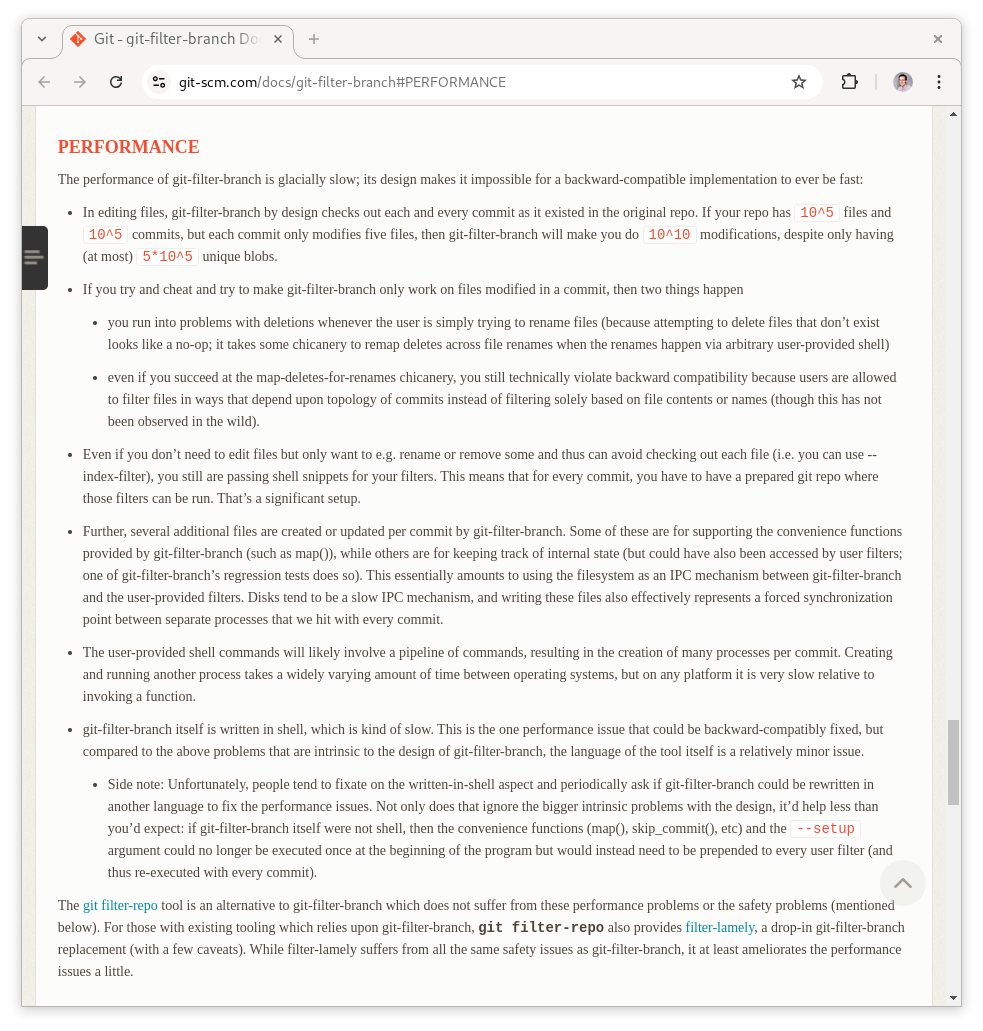
\includegraphics[scale=0.35]{git-filter-branch-manual-performance.png}
  }

  \only<6>{
  
\includegraphics[scale=0.35]{git-filter-branch-manual-safety.png}
  }

\end{frame}

\begin{comment}
%%%%%%%%%%%%%%%%%%%%%%%%%%%%%%%%%%%%%%%%%%%%%%%%%%%%%%%%%%%%%%%%%%%%%%%%%%

\begin{frame}
  \frametitle{Problems with existing solutions: git-filter-branch}

  git-filter-branch design issues:
  \begin{itemize}
    \item Checking out each version, or even creating an index of each version
    \item Using writing to disk as an IPC mechanism
    \item Forking millions of subprocesses
    \item Shell has all kinds of quoting issues \textit{and} portability issues
    \item Usability defaults are atrocious
  \end{itemize}

\end{frame}

%%%%%%%%%%%%%%%%%%%%%%%%%%%%%%%%%%%%%%%%%%%%%%%%%%%%%%%%%%%%%%%%%%%%%%%%%%

\begin{frame}
  \frametitle{Problems with existing solutions: BFG Repo Cleaner}

  How does BFG Repo Cleaner fare with these usecases?

  \only<2->{
  \vspace*{\baselineskip}

  It can't solve any of them, nor any portion of them.
  }

  \only<3->{
  \vspace*{\baselineskip}

  This isn't just a case of missing features; its design restricts it to
  the few problems it has already solved.  
  }

\end{frame}
\end{comment}

%%%%%%%%%%%%%%%%%%%%%%%%%%%%%%%%%%%%%%%%%%%%%%%%%%%%%%%%%%%%%%%%%%%%%%%%%%

\begin{frame}
  \frametitle{Problems with existing solutions: BFG Repo Cleaner}

  Unlike git-filter-branch, I have high respect for BFG Repo Cleaner.  It:
  \begin{itemize}
    \item is quick
    \item has some really nice design ideas (which \only<1-2>{I stole from liberally}\only<3->{\Red{I stole from liberally}})
    \item is a decent tool for the few usecases it can handle
  \end{itemize}

  \only<2->{
  \vspace*{0.5\baselineskip}
  BFG's fundamental shortcoming:
  \begin{itemize}
    \item Works by walking through packs and packed-refs files, meaning:
    \begin{itemize}
      \item must work on basenames (e.g. \texttt{README.md}) instead of full
            paths (e.g. \texttt{subdir/README.md})
            $\Rightarrow$ no restructuring workflows are possible
      \item Misses loose objects and loose refs when rewriting history
            (cf. \texttt{core.bigFileThreshold})
      \item doesn't update the working tree or index at end of rewrite,
            which has multiple knock-on usability effects
    \end{itemize}
  \end{itemize}
  }

  \only<4->{
  \vspace*{0.4\baselineskip}
  git-filter-repo supports roughly all the same flags as BFG with mostly
  the same meaning and same behavior.
  }

\end{frame}

%%%%%%%%%%%%%%%%%%%%%%%%%%%%%%%%%%%%%%%%%%%%%%%%%%%%%%%%%%%%%%%%%%%%%%%%%%
\subsection[Dieting]{Putting a repository on a diet}
%%%%%%%%%%%%%%%%%%%%%%%%%%%%%%%%%%%%%%%%%%%%%%%%%%%%%%%%%%%%%%%%%%%%%%%%%%

\begin{frame}
  \frametitle{Excising historical clutter erroneously committed}

  The final motivator: ancient, large historical cruft.  \only<2->{
  Unfortunately:

  \vspace*{\baselineskip}
  \begin{itemize}[<+->]
    \item The tools for finding this clutter were poor
    \item<3-> Most guides for doing this presupposed individual big blobs
    \item<4-> Individual big blobs only accounted for part of my estimate
          of unnecessary bloat
  \end{itemize}
  }

  \only<5->{
  \vspace*{\baselineskip}
  I found there were three sources:
  \begin{itemize}[<+->]
    \item<5-> Individual big blobs
    \item<6-> Certain extensions (e.g. tarballs, zipfiles, powerpoint slides,
          videos)
    \item<7-> Directories (e.g. node\_modules, bower\_components,
              autogenerated output)
  \end{itemize}
  }

\end{frame}

%%%%%%%%%%%%%%%%%%%%%%%%%%%%%%%%%%%%%%%%%%%%%%%%%%%%%%%%%%%%%%%%%%%%%%%%%%

\begin{frame}
  \frametitle{Excising historical clutter erroneously committed}

  \cl{git filter-repo {-}{-}analyze} \\

  \only<2->{
  \cl{ls .git/filter-repo/analysis} \\
  \texttt{
  \begin{tabular}{ll}
  blob-shas-and-paths.txt        & path-all-sizes.txt     \\
  directories-all-sizes.txt      & path-deleted-sizes.txt \\
  directories-deleted-sizes.txt  & README                 \\
  extensions-all-sizes.txt       & renames.txt            \\
  extensions-deleted-sizes.txt
  \end{tabular}
  }}

\end{frame}

%%%%%%%%%%%%%%%%%%%%%%%%%%%%%%%%%%%%%%%%%%%%%%%%%%%%%%%%%%%%%%%%%%%%%%%%%%

\begin{frame}[containsverbatim]

  \cl{less .git/filter-repo/analysis/path-all-sizes.txt} \\
  {\small
  \begin{verbatim}
=== All paths by reverse accumulated size ===
Format: unpacked size, packed size, date deleted, path name
   106605620    3735123 <present>  package-lock.json
    24875876    1937119 <present>  polymer.js.map
     1664408    1492053 2018-05-10 img/migration.png
     7252147     698756 2013-05-13 toolkit.min.js.map
    30747371     678832 <present>  CHANGELOG.md
     8463771     647405 <present>  polymer.js
     5165644     615251 2013-05-13 toolkit.native.min.js.map
     4486888     613498 2015-04-10 components/platform/platform.js.map
     3804736     550305 2013-06-19 polymer.native.min.js.map
     8219468     547671 <present>  bower_components/hydrolysis/hydrolysis.js
     5444644     479370 2013-06-19 polymer.min.js.map
     2462896     371935 2013-06-19 polymer.sandbox.min.js.map
     5832454     349154 <present>  polymer.html
     2296880     327724 2014-11-17 web-component-tester/browser.js
      316011     315266 2014-11-13 projects/pica/assets/fashion.jpg
  \end{verbatim}
  }

\end{frame}

%%%%%%%%%%%%%%%%%%%%%%%%%%%%%%%%%%%%%%%%%%%%%%%%%%%%%%%%%%%%%%%%%%%%%%%%%%

\begin{frame}[containsverbatim]

  \cl{less .git/filter-repo/analysis/extensions-all-sizes.txt} \\
  {\small
  \begin{verbatim}
=== All extensions by reverse size ===
Format: unpacked size, packed size, date deleted, extension name
   173415935    7675374 <present>  .html
    91831815    5787794 <present>  .js
    54922739    5431038 <present>  .map
   107306538    3813602 <present>  .json
     2454855    2443945 2016-09-08 .jpg
     2000382    1787159 2018-05-10 .png
    42258642    1122429 <present>  .md
     2600878     259034 <present>  .ts
     1784410     160552 <present>  .log
      185311     154039 2016-09-08 .vsdx
       53975      54233 2014-12-12 .gz
      329208      48362 <present>  .css
      219273      26234 2015-05-15 .svg
       62798      17236 2015-04-08 .bak
       42734      13469 <present>  <no extension>
  \end{verbatim}
  }

\end{frame}

%%%%%%%%%%%%%%%%%%%%%%%%%%%%%%%%%%%%%%%%%%%%%%%%%%%%%%%%%%%%%%%%%%%%%%%%%%

\begin{frame}[containsverbatim]

  \cl{less .git/filter-repo/analysis/directories-all-sizes.txt} \\
  {\small
  \begin{verbatim}
=== All directories by reverse size ===
Format: unpacked size, packed size, date deleted, directory name
   479554929   28813077 <present>  <toplevel>
    51117672    3215151 <present>  src
    79087157    2634500 <present>  test
     2862175    2429111 2014-11-19 projects
    15208313    2131570 2015-04-10 components
    73658545    2100858 <present>  test/unit
    60958535    1983043 <present>  lib
     1529788    1513749 2014-11-19 projects/spa
     1515069    1510233 2014-11-19 projects/spa/assets
     1664408    1492053 2018-05-10 img
    12027824    1106822 <present>  bower_components
    40641208    1013850 <present>  lib/mixins
    13884241     960879 <present>  src/lib
      963127     815654 2014-11-19 projects/pica
      816153     795333 2014-11-19 projects/pica/assets
  \end{verbatim}
  }

\end{frame}

%%%%%%%%%%%%%%%%%%%%%%%%%%%%%%%%%%%%%%%%%%%%%%%%%%%%%%%%%%%%%%%%%%%%%%%%%%
\section[Usecases]{Sampling of other capabilities/usecases}
\subsection[Paths]{Slicing and dicing by paths}
%%%%%%%%%%%%%%%%%%%%%%%%%%%%%%%%%%%%%%%%%%%%%%%%%%%%%%%%%%%%%%%%%%%%%%%%%%

\begin{frame}
  \frametitle{Slicing and dicing by paths}

  Remove a few paths\\
  \cl{git filter-repo {-}{-}invert-paths {-}{-}path bad/path1 $\backslash$\\
  \quad\qquad {-}{-}path src/mod/subdir/}\\

  \pause
  \vspace*{0.75\baselineskip}
  Remove all files with a certain extension\\
  \cl{git filter-repo {-}{-}invert-paths {-}{-}path-glob \textquotesingle{}*.mp4\textquotesingle{}}\\

  \pause
  \vspace*{0.75\baselineskip}
  Specify a (long) list of files or directories to keep (removing everything else)\\
  \cl{git filter-repo {-}{-}paths-from-file list-of-files.txt}\\

\end{frame}

%%%%%%%%%%%%%%%%%%%%%%%%%%%%%%%%%%%%%%%%%%%%%%%%%%%%%%%%%%%%%%%%%%%%%%%%%%

\begin{frame}[containsverbatim]
  \frametitle{Slicing and dicing by paths}

  {\footnotesize
  \cl{git filter-repo {-}{-}paths-from-file /tmp/path-rules.txt}\\
  where\\
  \cl{cat /tmp/path-rules.txt}\\
  \begin{verbatim}
# Keep these file or directory paths (similar to --path):
README.md
guides/how-to-start.txt
tools/releases/

# Keep files matching this glob (similar to --path-glob):
glob:*.py

# Keep files matching this regex (similar to --path-regex):
regex:^.*/.*/[0-9]{4}-[0-9]{2}-[0-9]{2}.txt$

# An example of renaming a path
tools/==>scripts/

# An example of using a regex to rename a path
regex:(.*)/([^/]*)/([^/]*)\.text$==>\2/\1/\3.txt
  \end{verbatim}
  }

\end{frame}

%%%%%%%%%%%%%%%%%%%%%%%%%%%%%%%%%%%%%%%%%%%%%%%%%%%%%%%%%%%%%%%%%%%%%%%%%%

\begin{frame}
  \frametitle{Slicing and dicing by paths}

  Using a function callback; remove all filenames with backslashes:\\
  \cl{git filter-repo {-}{-}filename-callback "\\
  \quad\qquad return None if \textquotesingle{}$\backslash\backslash$\textquotesingle{} in filename else filename"}\\

  \pause
  \vspace{0.75\baselineskip}
  NFD/NFC conversion in filenames\\
  \cl{git filter-repo {-}{-}filename-callback \textquotesingle{}\\
  \quad\qquad cmd = "iconv -f utf-8-mac -t utf-8".split()\\
  \only<2>{
  \quad\qquad return subprocess.check\_output(cmd,
                                   input=filename)\textquotesingle{}\\
  }
  \only<3->{
  \quad\qquad \Red{try:}\\
  \quad\qquad\quad return subprocess.check\_output(cmd, input=filename)\\
  \quad\qquad \Red{except:\\
  \quad\qquad\quad return filename}\textquotesingle{}\\
  }
  }

\end{frame}

%%%%%%%%%%%%%%%%%%%%%%%%%%%%%%%%%%%%%%%%%%%%%%%%%%%%%%%%%%%%%%%%%%%%%%%%%%
\subsection[Replace]{Using replace objects}
%%%%%%%%%%%%%%%%%%%%%%%%%%%%%%%%%%%%%%%%%%%%%%%%%%%%%%%%%%%%%%%%%%%%%%%%%%

\begin{frame}
  \frametitle{Other history rewrite types}

  Deleting all history prior to a given commit (basically squashing all
  prior history into that commit):\\
  \cl{git replace {-}{-}graft \$\{OLD\_COMMIT\}}\\
  \cl{git filter-repo {-}{-}proceed}\\

  \only<2->{
  \vspace*{\baselineskip}
  This \texttt{git replace} trick above can also be used to fix individual
  corrupt objects; git replace can be used to create a replacement commit
  modifying any of
  \begin{itemize}[<+->]
    \item<3-> parents (as done above)
    \item<4-> bad timezone
    \item<5-> missing author email
    \item<6-> etc.
  \end{itemize}
  \only<7->{
  \texttt{git filter-repo} takes local replace refs and rewrites commits in
  history to make the change permanent.
  }}

\end{frame}

%%%%%%%%%%%%%%%%%%%%%%%%%%%%%%%%%%%%%%%%%%%%%%%%%%%%%%%%%%%%%%%%%%%%%%%%%%
\subsection[Text]{Replacing file text}
%%%%%%%%%%%%%%%%%%%%%%%%%%%%%%%%%%%%%%%%%%%%%%%%%%%%%%%%%%%%%%%%%%%%%%%%%%

\begin{frame}[containsverbatim]
  \frametitle{Replacing text}

  Replace text found in non-binary files found throughout the repository:\\
  \cl{cat /tmp/expressions.txt}\\
  {\footnotesize
  \begin{verbatim}
p455w0rd
foo==>bar
glob:*666*==>
regex:\bdriver\b==>pilot
literal:MM/DD/YYYY==>YYYY-MM-DD
regex:([0-9]{2})/([0-9]{2})/([0-9]{4})==>\3-\1-\2
  \end{verbatim}
  }
  \vspace*{-0.5\baselineskip}
  \cl{git filter-repo {-}{-}replace-text /tmp/expressions.txt}\\

\end{frame}

%%%%%%%%%%%%%%%%%%%%%%%%%%%%%%%%%%%%%%%%%%%%%%%%%%%%%%%%%%%%%%%%%%%%%%%%%%

\begin{frame}[containsverbatim]
  \frametitle{Replacing text}

  Replace text found in non-binary files found throughout the repository:\\
  \cl{cat /tmp/expressions.txt}\\
  {\footnotesize
  \begin{verbatim}
p455w0rd
foo==>bar
glob:*666*==>
regex:\bdriver\b==>pilot
literal:MM/DD/YYYY==>YYYY-MM-DD
regex:([0-9]{2})/([0-9]{2})/([0-9]{4})==>\3-\1-\2
  \end{verbatim}
  }
  \vspace*{-0.5\baselineskip}
  \cl{git filter-repo {-}{-}replace-text /tmp/expressions.txt}\\

  \vspace*{\baselineskip}
  There is also a  {-}{-}replace-messages, similar to {-}{-}replace-text, for
  updating commit messages rather than file contents.

\end{frame}

%%%%%%%%%%%%%%%%%%%%%%%%%%%%%%%%%%%%%%%%%%%%%%%%%%%%%%%%%%%%%%%%%%%%%%%%%%

\begin{frame}
  \frametitle{..and many more}

  \vfill
  \texttt{git-filter-repo} has many additional flags for rewriting
  history in various ways.
  \pause
  \vfill
  git-filter-repo can also be used as a library that is imported and used
  to write completely new filtering programs
  \pause
  , such as:
  \begin{itemize}
    \item git-filter-branch rewrite from scratch (\texttt{filter-lamely})
    \item bfg rewrite from scratch (\texttt{bfg-ish})
  \end{itemize}

  %sensitive data removal

\end{frame}

%%%%%%%%%%%%%%%%%%%%%%%%%%%%%%%%%%%%%%%%%%%%%%%%%%%%%%%%%%%%%%%%%%%%%%%%%%

\subsection{}
\begin{frame}
  \vfill
  {\Huge
  \begin{center}I hope you rarely ever need to use history rewriting tools...\end{center}
  \vfill
  \only<1>{
  \begin{center}{\color{MyWhite}invisible text of enough length to take up the same space}\end{center}}
  \only<2->{
  \begin{center}but if you do, that git-filter-repo comes in very handy.\end{center}}
  }
  \vfill
\end{frame}

%%%%%%%%%%%%%%%%%%%%%%%%%%%%%%%%%%%%%%%%%%%%%%%%%%%%%%%%%%%%%%%%%%%%%%%%%%

\end{document}
